\section{Introduction}

%\begin{itemize}
%\item Tuning is important in deep learning and tuning is hard.
%\item People do (a) adaptive (b) method with knob. (Fix momentum and only investigate lr).
%\item momentum accelerates. better understanding the behavior of momentum is interesting better tuner with less tuning. We revisit mom sgd and found the robustness to lr and variation. As well as related to async. And derive simple theory to analyze. 
%\item These properties makes mom sgd a good candidate for auto tuning. We investigate a quadratic model and propose an simple and easy to understand tuner. It is faster than Adam
%\item We also connect to async theory and develope component and better than others in asynchrony.  
%\end{itemize}

\outline{[Problem.]}
%Deep learning involves the use of very large datasets to fit large, complex models.
Accelerated forms of stochastic gradient descent (SGD), pioneered by
\citet{polyak1964some} and \citet{nesterov1983method}, are the de-facto
training algorithms for deep learning.
Their use requires a sane choice for their {\em hyperparameters}: 
typically a {\em learning rate} and {\em momentum parameter} \citep{sutskever2013importance}.
\outline{[Hardness.]}
%Hyperparameter tuning is often cited as being the number-one factor in extracting good performance from deep learning systems. 
%It is by far the most time consuming phase of developing a new deep learning model or system.
%One could say that tuning is {\em the hidden cost of modern machine learning},
However, tuning hyperparameters is arguably the most time-consuming part of deep learning, with thousands of grad-student-hours sacrificed and many papers outlining best tuning practices written
\cite{bengio2012practical,orr2003neural,bengio2012deep,bottou2012stochastic}.

\outline{[previous approach]}
Deep learning researchers have proposed a number of methods to deal with hyperparameter optimization. 
Na\"ive methods, like the grid-search,
are prohibitively expensive for all but the smallest problems. 
Smart black-box methods \cite{bergstra2012random,snoek2012practical}
do not explicitly take into account the problem specifics and spend time testing multiple configurations.
Adaptive methods provide an attractive alternative.
They aim to tune a single run on the fly and have been largely successful in relieving practitioners of tuning the learning rate. 
Algorithms like Adagrad \cite{duchi2011adaptive}, RMSProp \cite{tieleman2012lecture} and Adam \cite{kingma2014adam} use the magnitude of gradient elements to tune learning rates {\em individually for each variable}. A common limitation of state-of-the-art adaptive methods is that they do not tune their momentum.
%Finally, methods like the one proposed by \citet{schaul2013no} use simple models and simple measurements to tune a global learning rate for the standard SGD update.

\outline{[limitation of previous approach]}
Momentum is a fundamental parameter at the heart of the acceleration process, lending its name to the most ubiquitous accelerated method \cite{polyak1964some}, simply dubbed {\em momentum}.
Classic \cite{polyak1964some} and recent results \cite{sutskever2013importance} alike show that proper momentum tuning has a significant impact on training speed. 
%Unfortunately, there exists no method that automatically tunes its momentum parameter.
%Large-scale systems pose extra tuning challenges.
\jianedits{Momentum becomes even more critical on distributed systems. 
Recently, \citet{mitliagkas2016asynchrony} showed that, in asynchronous-parallelization~\cite{recht2011hogwild,dean2012large,chilimbi2014project,hadjis2016omnivore},
a technique for efficient distributed training without synchronization locks, 
%introduces additional momentum-like dynamics to momentum SGD, and
one can manually reduce algorithmic momentum to accelerate convergence~\cite{hadjis2016omnivore}.
As part of a collaboration with an industry affiliate and a big research lab, we verify that tuning momentum dramatically improves convergence on thousand-node scales.
However, grid-searching momentum on very large cluster jobs becomes especially challenging.
We believe that better understanding of momentum and its rich properties is interesting in its own right and could yield a next generation of adaptive methods that perform {\em automatic momentum tuning}. }
%Increasing model and dataset sizes motivate parallelization \cite{dean2012large,chilimbi2014project,hadjis2016omnivore,chen2016revisiting}.
% Asynchronous methods \cite{recht2011hogwild} provide efficient parallelization by training without locking or synchronization.
%The exact effect of asynchrony on the optimization process has been a mystery, though empirical results have shown great successes \cite{recht2011hogwild,dean2012large,chilimbi2014project,hadjis2016omnivore}.
%Recent work by \citet{mitliagkas2016asynchrony} reveals that asynchrony introduces additional momentum-like dynamics to the optimization process,
%a statement that can be made {\em exact} for the momentum SGD algorithm.
%\jianedits{Recent work by \citet{mitliagkas2016asynchrony} reveals that asynchrony introduces additional momentum-like dynamics to momentum SGD, and one can manually reduce algorithmic momentum to accelerate convergence~\cite{hadjis2016omnivore}}.

%As part of a collaboration with an industry affiliate and a big research lab, we had the opportunity to verify this phenomenon on thousand-node scales.
%Tuning the momentum value improves convergence speed,
%however grid-searching momentum values at that scale becomes challenging.
%Recent work \cite{hadjis2016omnivore} uses this theoretical understanding to perform targeted, efficient hyperparameter searches.
%We believe that better understanding of momentum and its rich properties is interesting in its own right and could yield a next generation of adaptive methods with {\em automatic momentum tuning}.


%%%%%%%% old un smoothed version %%%%%%%%%%%%%%%%%%
%%Large-scale systems pose extra tuning challenges.
%Momentum tuning becomes even more critical on large-scale, parallel systems.
%%Increasing model and dataset sizes motivate parallelization \cite{dean2012large,chilimbi2014project,hadjis2016omnivore,chen2016revisiting}.
% Asynchronous methods \cite{recht2011hogwild} provide efficient parallelization by training without locking or synchronization.
%The exact effect of asynchrony on the optimization process has been a mystery, though empirical results have shown great successes \cite{recht2011hogwild,dean2012large,chilimbi2014project,hadjis2016omnivore}.
%%Recent work by \citet{mitliagkas2016asynchrony} reveals that asynchrony introduces additional momentum-like dynamics to the optimization process,
%%a statement that can be made {\em exact} for the momentum SGD algorithm.
%\jianedits{Recent work by \citet{mitliagkas2016asynchrony} reveals that asynchrony introduces additional momentum-like dynamics to momentum SGD, and one can manually reduce algorithmic momentum to accelerate convergence~\cite{hadjis2016omnivore}}.
%
%As part of a collaboration with an industry affiliate and a big research lab, we had the opportunity to verify this phenomenon on thousand-node scales.
%Tuning the momentum value improves convergence speed,
%however grid-searching momentum values at that scale becomes challenging.
%Recent work \cite{hadjis2016omnivore} uses this theoretical understanding to perform targeted, efficient hyperparameter searches.
%We believe that better understanding of momentum and its rich properties is interesting in its own right and could yield a next generation of adaptive methods that also perform {\em automatic momentum tuning}.
%%%%%%%%%%%%%%%%%%%%%%%%%%%%%%%%%%%%%%%%%%%%%%%%%%%


\begin{wrapfigure}[11]{R}{0.46\textwidth}
\vspace{-1.0em}
\begin{minipage}{1.0\linewidth}
\begin{figure}[H]
	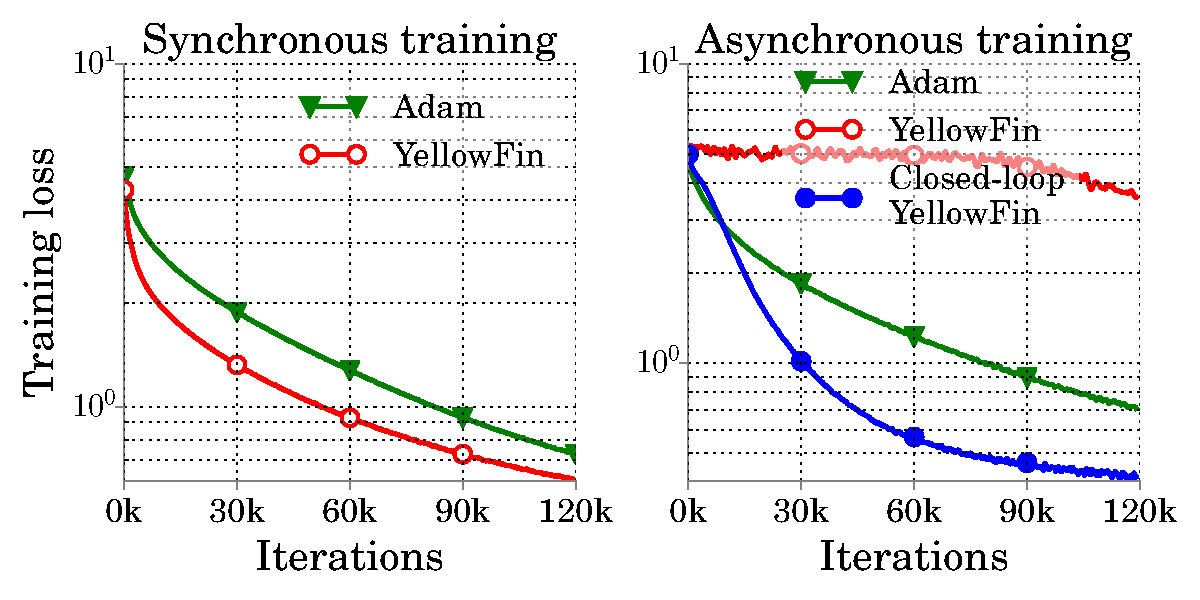
\includegraphics[width=1.0\linewidth]{experiment_results/spotlight.pdf}
	\caption{\tuner comparing to Adam.}
\end{figure}
\end{minipage}
\end{wrapfigure}
We revisit the basic SGD update that uses Polyak's momentum and a single learning rate for all variables.
We empirically show that, when hand-tuned, momentum SGD achieves faster convergence than Adam for a large class of models.
We then formulate the optimization update as a dynamical system and study certain robustness properties of the momentum operator.
Building on our analysis, we design \tuner, an automatic hyperparameter tuner for momentum SGD.
\tuner tunes the learning rate and momentum on the fly, and uses a novel {\em closed-loop control architecture} to compensate for the added dynamics of asynchrony.
Specifically:
\begin{itemize}[leftmargin=2em]
\item
The momentum operator's spectral radius is constant in a large subset of the hyperparameter space we call {\em the robust region}.
This is a known, but relatively obscure property.
Our analysis in Section~\ref{sec:momentum_operator} gives a novel interpretation:
momentum is robust to learning rate misspecification and curvature variation,
two desirable properties for deep learning.
%\item 
%We analyze the momentum operator in Section~\ref{sec:momentum_operator} with focus on its spectral radius. More specifically, the spectral radius can be constant under conditions.
%We expose previously unknown insights from the simple property: 
%the momentum operator can yield constant convergence rates even when the learning rate is grossly mis-tuned.
%Furthermore, constant convergence rates are empirically possible for some non-convex objectives,
%where curvature dramatically varies spatially.%  (a factor of more than $1000\times$ when momentum is set to $0.9$).
\item
In Section~\ref{sec:sync_tuner}, we use these insights and a simple quadratic model analysis to design \tuner, an automatic tuner for momentum SGD.
\tuner uses on-the-fly measurements from the gradients of the system to tune both learning rate and momentum.
%\item We use these insights and the analysis of a quadratic model to design
%\tuner in Section~\ref{sec:sync_tuner}. To tune the learning rate and momentum, the tuner minimize the squared distance from the minimum of a local quadratic approximation at each step of the algorithm.
%\item In Section~\ref{sec:async_tuner}, we present the first asynchrony-aware tuner. 
%We first provide a measurement component to estimate the total amount of momentum in a running system, including the extra momentum due to asynchrony.  
%Then, we propose \asynctuner, a closed-loop version of \tuner, that uses the measurement component and a negative feedback loop to bring the total amount of momentum to the levels suggested by the tuning rule.
%\item 
%Furthermore, \tuner is {\em asynchrony-aware}. 
%It uses a {\em novel momentum-measurement mechanism} that is part of a {\em closed-loop} design to automatically tune the value of momentum when asynchrony introduces extra momentum dynamics.
\item In Section~\ref{sec:async_tuner}, we present \asynctuner 
%an asynchrony-aware tuner. 
\jianedits{for asynchronous training}.
\jianedits{It} measures the total momentum in a running system, including any asynchrony-induced momentum. 
This measurement is used in a negative feedback loop to control the value of algorithmic momentum.% on the fly.
%With the estimates, it use a negative feedback loop to bring the total momentum to the level suggested by \asynctuner.

%\item We present an analysis of the momentum operator in Section~\ref{sec:momentum_operator}.
%We focus on the fact that its spectral radius is constant in a certain robust region.
%We expose previously unknown insights that stem from that simple property: 
%the momentum operator can yield constant convergence rates even when the learning rate is grossly mis-tuned.
%Furthermore, constant convergence rates are possible for certain non-convex objectives,
%where curvature can vary dramatically (a factor of more than $1000\times$ when momentum is set to $0.9$).
\end{itemize}

%Asynchronous methods \cite{recht2011hogwild} provide very efficient parallelization by doing away with locking and synchronization.

%and propose \tuner, an automatic tuner for its hyperparameters.
%A key component of \tuner is principled momentum-tuning in both synchronous and asynchronous settings.
%\tuner is competitive or better that state-of-the-art adaptive methods and is asynchrony-aware by using a novel design based on measuring the level of momentum on the fly and using a closed-loop control module for momentum.

%\outline{[OUR RESULTS]}
%We demonstrate experimentally, in Section~\ref{sec:experiments}, that
%for a large class of networks, hand-tuned momentum SGD is competitive with Adam ($0.88-1.82\times$), even though it uses fixed hyperparameters throughout execution.
%On ResNets, momentum SGD can achieve a $1.25-1.82\times$ speedup over Adam.
%\tuner is competitive with, and sometimes better, than state-of-the-art adaptive methods. The speedup is over $2\times$ on ResNets and $1.18\times$ on LSTMs.
%Other adaptive algorithms do not tune their momentum parameter and suffer, as a result, in asynchronous settings.
%Hand-tuning momentum for Adam can improve its convergence rate by up to $2\times$, when using $16$ asynchronous workers. 
%Finally, closing the momentum loop in \tuner yields a speedup of $1.3-3\times$, when using $16$ asynchronous workers.
%Closed-loop \tuner achieves a speedup of about $2.7\times$ over Adam on 16 asynchronous workers.
%\begin{itemize}
%\item For a large class of networks, hand-tuned momentum SGD is competitive with Adam ($0.88-1.82\times$), even though it uses fixed hyperparameters throughout execution.
%On ResNets, momentum SGD can achieve a $1.25-1.82\times$ speedup over Adam.
%\item \tuner is competitive with, and sometimes better, than state-of-the-art adaptive methods. The speedup is over $2\times$ on ResNets and $1.18\times$ on LSTMs.
%\item  Other adaptive algorithms do not tune their momentum parameter and suffer, as a result, in asynchronous settings.
%Hand-tuning momentum for Adam can improve its convergence rate by up to $2\times$, when using $16$ asynchronous workers.
%\item  Closing the momentum loop in \tuner yields a speedup of $1.3-3\times$, when using $16$ asynchronous workers.
%Closed loop \tuner achieves a speedup of about $2.7\times$ over Adam on 16 asynchronous workers.
%\end{itemize}


\outline{[empirical performance statement on \tuner]}
We introduce our contributions in Sections~\ref{sec:momentum_operator},\ref{sec:sync_tuner},\ref{sec:async_tuner}.
In Section~\ref{sec:experiments}, we demonstrate empirically that 
\tuner offers \jianedits{competitive or significantly better performance} compared to:
(i) hand-tuned momentum SGD (a speedup of up to 2.3x);
and (ii) hand-tuned Adam (up to 2.8x speedup).
	\jianedits{In an asynchronous setting, we demonstrate that Adam, the state-of-the-art adaptive method, suffers from lack of momentum tuning.}
%Specifically, when we hand-tune Adam's momentum, its asynchronous performance improves by at least 2.5x.
In the same setting, the closed-loop control architecture speeds up \tuner by up to 2x, 
%closing \tuner's momentum loop improves its performance by 1.5x-3x.
\jianedits{allowing \Asynctuner to outperform Adam with a more than 2.7x speedup}.
\jianedits{As a conclusion, we present related work in Section~\ref{sec:related} and discussion in Section~\ref{sec:discussion}.}
%We conclude with related work in Section~\ref{sec:related} and discussion in Section~\ref{sec:discussion}

%We introduce our contributions in Sections~\ref{sec:momentum_operator},\ref{sec:sync_tuner},\ref{sec:async_tuner}.
%Section~\ref{sec:experiments} gives experimental validation of our claims and we conclude with related work in Section~\ref{sec:related} and discussion in Section~\ref{sec:discussion}.
